\documentclass[aspectratio=43]{beamer}

\usepackage[french]{babel}
\usepackage{caption}
\usepackage[T1]{fontenc}
\usepackage{amsmath, amsfonts, amssymb, mathtools}
\usepackage{stmaryrd}
\usepackage{fancyhdr}
\usepackage{lipsum}
\usepackage{graphicx}
\usepackage[ddmmyyyy]{datetime}
\usepackage{adjustbox}
\usepackage[explicit]{titlesec}
\usepackage{pdfpages}

\usetheme{Madrid}

\definecolor{white}{gray}{0.98}
\definecolor{green}{HTML}{92D050}
\usefonttheme[onlymath]{serif}

\makeatletter
\definecolor{beamer@blendedblue}{HTML}{3294A8} % changed this


\title[Compression]{TIPE - LA COMPRESSION DE DONN\'EES}
\subtitle{Et son application aux images}
\author{Ars\`ene MALLET}
\date[\today]{\today}
\institute{Candidat - 14873}

\begin{document}


\begin{frame}
    \titlepage
\end{frame}

\begin{frame}
    \frametitle{Introduction}

    \begin{itemize}
        \setlength\itemsep{2em}
        \item \Large \textbf{Compression} : \textcolor{red}{maximum} d'information avec une taille \textcolor{green}{minimal}
        \item Deux types : \textbf{avec} (lossy) ou \textbf{sans} perte (lossless).
        \item \large Dans le domaine urbain : beaucoup d'information $\rightarrow$ compression $\Rightarrow$ \bfseries stocker et traiter efficacement
    \end{itemize}

\end{frame}

\begin{frame}
    \frametitle{Proc\'ed\'es de Compression}

    \begin{itemize}
        \Large
        \setlength\itemsep{2em}
        \item Compression sans perte : \textbf{entropique} et \textbf{algorithmique}
        \item Une \textbf{réorganisation} des données
        \item Application de \textbf{transformées mathématiques}
        \item Implémentation de l'\textbf{algorithme JPEG}
    \end{itemize}

\end{frame}

\begin{frame}
    \frametitle[allowframebreaks]{Entropie et Codage Optimal (1)}

    \begin{block}{Th\'eorie de l'Information de Shannon}
        Théorie probabiliste \textbf{quantifiant l’information} d’un ensemble de messages.
    \end{block}
    
    \vspace*{1em}

    \begin{alertblock}{Définition - Entropie}
        Pour une source $X$ comportant $n$ symboles, un symbole $x_i$ ayant
        une probabilité $p_i = \mathbb{P}(X = x_i)$ d’apparaître, l'entropie $H$ est définie par : 
        $$ H(X) = - \sum_{i = 1}^{n} p_i \log_2 (p_i) $$
    \end{alertblock}
\end{frame}

\begin{frame}
    \frametitle{Entropie et Codage Optimal (2)}

    \begin{alertblock}{Définition - \bfseries Code de Source}
        Un \textbf{code de source C} pour une variable aléatoire $X$ de distribution de probabilité $p$, est une application de $\Omega$ (ensemble des symboles sources) vers $A^*$
        (où $A$ est l'alphabet du code).
    \end{alertblock}

    \vspace*{2em}

    \begin{alertblock}{Définition - Code \bfseries Uniquement Décodable}
        Un code est dit \textbf{uniquement décodable} si
        $$ \forall x, y \in \Omega^+, \; x \neq y \implies C^+(x) \neq C^+(y)$$
    \end{alertblock}
\end{frame}
    
\begin{frame}
    \frametitle{Entropie et Codage Optimal (3)}

    \begin{alertblock}{Définition - Code \bfseries Préfixe}
        Un code est dit préfixe si \textbf{aucun mot de code n'est le préfixe d'un autre mot} de code
    \end{alertblock}

    \textit{Rq. :} Code \textbf{préfixe} $\implies$ \textbf{code uniquement décodable}

    \vspace*{3em}

    \begin{columns}
        \begin{column}{0.5\textwidth}
            \centering 
            Un code \bfseries non-préfixe \\
            \begin{tabular}{c | c}
                \hline
                $a$ & $0$ \\
                $b$ & $1$ \\
                $c$ & $01$ \\ \hline
            \end{tabular} \\
        \vspace*{1em}
        $ab = 01 = c \rightarrow$ \textbf{\alert{Non} uniquement décodable}
        \end{column}

        \begin{column}{0.5\textwidth} %%
            \centering
            Un code \textbf{préfixe} \\
            \begin{tabular}{c | c}
                \hline
                $a$ & $0$ \\
                $b$ & $10$ \\
                $c$ & $11$ \\ \hline
            \end{tabular} \\
            \vspace*{1em}
            Chaque code est \textbf{unique}
        \end{column}
    \end{columns}
\end{frame}

\begin{frame}
    \frametitle{Entropie et Codage Optimal (4)}

    \begin{block}{Inégalité de Kraft}
        Pour un code défini sur un alphabet de taille D, et un alphabet de source $\Omega$ de taille 
$|\Omega|$, alors il est \textbf{préfixé} si et seulement si $$\sum _{{i=1}}^{{|\Omega |}}D^{{-l_{i}}}\leq 1$$
$l_i =$ longueur des mots du codes
    \end{block}

    \vspace*{2em}

    \begin{alertblock}{Théorème du Codage de Source - Shannon 1948}
        Lorsque l'efficacité de la compression augmente, la longueur moyenne du code tend vers l'entropie $H$.
    \end{alertblock}
    
\end{frame}

\begin{frame}
    \frametitle{Codage De Huffman (1)}

    \begin{columns}
        \begin{column}{0.5\textwidth}
            \centering

            \begin{itemize}
                \item Codage \textbf{optimal} au niveau \textbf{symbole}, à longueur \textbf{variable}
                \item Impose un \textbf{nombre entier de bit} pour un symbole
                \item Exemple de codage de \\ "LES VILLES" :
            \end{itemize}

            \vspace*{2em}

            \begin{tabular}{c | c}
                symbole source & fréquence \\
                \hline
                L & $3$ \\
                E & $2$ \\
                S & $2$ \\
                V & $1$ \\
                I & $1$ \\ \hline
            \end{tabular}
        \end{column}

        \begin{column}{0.5\textwidth}
            \textbf{Arbre de Huffman} de "LES VILLES"

            \vspace*{2em}

            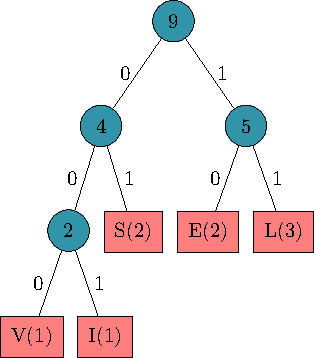
\includegraphics{img/huffmanExample/huffmanExample.pdf}
        \end{column}
    \end{columns}
\end{frame}

\begin{frame}
    \frametitle{Codage De Huffman (2)}

    \begin{columns}

        \begin{column}{0.5\textwidth}
            \textbf{Arbre de Huffman} de "LES VILLES"

            \vspace*{2em}

            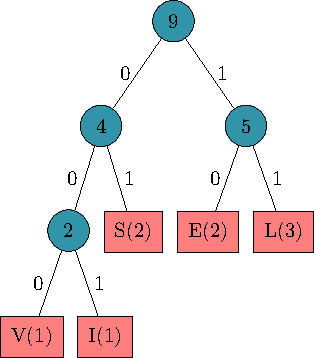
\includegraphics{img/huffmanExample/huffmanExample.pdf}
        \end{column}

        \begin{column}{0.5\textwidth}
            \centering

            \begin{itemize}
                \item \textbf{Table de code} de Huffman

            \vspace*{1em}

            \begin{tabular}{c | c}
                symbole source & code \\
                \hline
                L & $11$ \\
                E & $10$ \\
                S & $01$ \\
                V & $000$ \\
                I & $001$ \\ \hline
            \end{tabular}
            
            \vspace*{2em}

            \item \textbf{Code} de Huffman : $11100100000111111001$
        \end{itemize}

        \end{column}
    \end{columns}
\end{frame}

\begin{frame}
    \frametitle{Codage Arithmétique (1)}

    \begin{itemize}
        \item Codage \textbf{optimal} au niveau \textbf{bit}, à longueur \textbf{variable}
        \item Principe : codage \textbf{par morceaux} et non par symbole (Huffman)
        \item Exemple de codage de "VILLE":
    \end{itemize}

    \vspace*{1em}
    
    {
    \centering
    \begin{tabular}{c | c | c}
        symbole source & probabilité & intervalle  \\
        \hline
        V & $1/5$ & $[0; 0,2[$ \\ 
        I & $1/5$ & $[0,2; 0,4[$\\
        L & $2/5$ & $[0,4; 0,8[$\\
        E & $1/5$ & $[0,8; 1[$\\ \hline
    \end{tabular}\par
    }

    \vspace*{1em}

    \textbf{Ajout} d'un symbole $s$: \\
    \begin{enumerate}
        \item $BB = BS - BI$
        \item $BS \leftarrow BI + BB \times BS_s$
        \item $BI \leftarrow BI + BB \times BI_s$
    \end{enumerate}

\end{frame}

\begin{frame}
    \frametitle{Codage Arithmétique (2)}

    {
    \centering
    \begin{tabular}{c | c | c}
        symbole source & probabilité & intervalle  \\
        \hline
        V & $1/5$ & $[0; 0.2[$ \\ 
        I & $1/5$ & $[0.2; 0.4[$\\
        L & $2/5$ & $[0.4; 0.8[$\\
        E & $1/5$ & $[0.8; 1[$\\ \hline
    \end{tabular}\par
    }
    
    \vspace*{1em}

    Ajout de $s = $ V : \\
    $BS = BB = 1$, $BI = 0$, $BS_s = 0.2,\; BI_s = 0$ \\
    $BS \leftarrow 0 + 1 \times 0.2 = 0.2$ \\
    $BI \leftarrow 0 + 1 \times 0 = 0$ \\

    \vspace*{1em}

    Ajout, ensuite, de $s'=$ I : \\
    $BS = BB = 0.2$, $BI = 0$, $BS_{s'} = 0.4, \; BI_{s'} = 0.2$ \\
    $BS \leftarrow 0 + 0.2 \times 0.4 = 0.08$ \\
    $BI \leftarrow 0 + 0.2 \times 0.2 = 0.04$ \\

    \vspace*{0.5em}

    \dots
\end{frame}

\begin{frame}
    \frametitle{Codage Arithmétique (3)}

    {
    \centering
    \begin{tabular}{c | c | c}
        symbole source & probabilité & intervalle  \\
        \hline
        V & $1/5$ & $[0; 0.2[$ \\ 
        I & $1/5$ & $[0.2; 0.4[$\\
        L & $2/5$ & $[0.4; 0.8[$\\
        E & $1/5$ & $[0.8; 1[$\\ \hline
    \end{tabular}\par
    }

    \vspace*{1em}

    Code de "VILLE" : $x \in [0.06752 ; 0.0688]$ \\
    Par exemple $x = 0.068$ fonctionne.

    \vspace*{1em}

    \textbf{Décompression}: \\
    \begin{enumerate}
        \item $x \in [0; 0.2] \rightarrow$ V
        \item $x \leftarrow \frac{x - BI_V}{p_V} = 0.34$
        \item $x \in [0.2; 0.4] \rightarrow$ VI
        \item $x \leftarrow \frac{x - BI_I}{p_I} = 0.7$
        \item [\dots] 
        \item Mot \textbf{décodé} : VILLE
    \end{enumerate}

\end{frame}

\begin{frame}
    \frametitle{La Représentation d'Image}

    \centering

    Image = $\begin{pmatrix}
        (r,g,b)_{1,1} & \dots & (r, g, b)_{1,p} \\
        \vdots & \ddots & \vdots \\
        (r,g,b)_{n, 1} & \dots & (r, g, b)_{n, p} \\
    \end{pmatrix}$

    \vspace*{2em}

    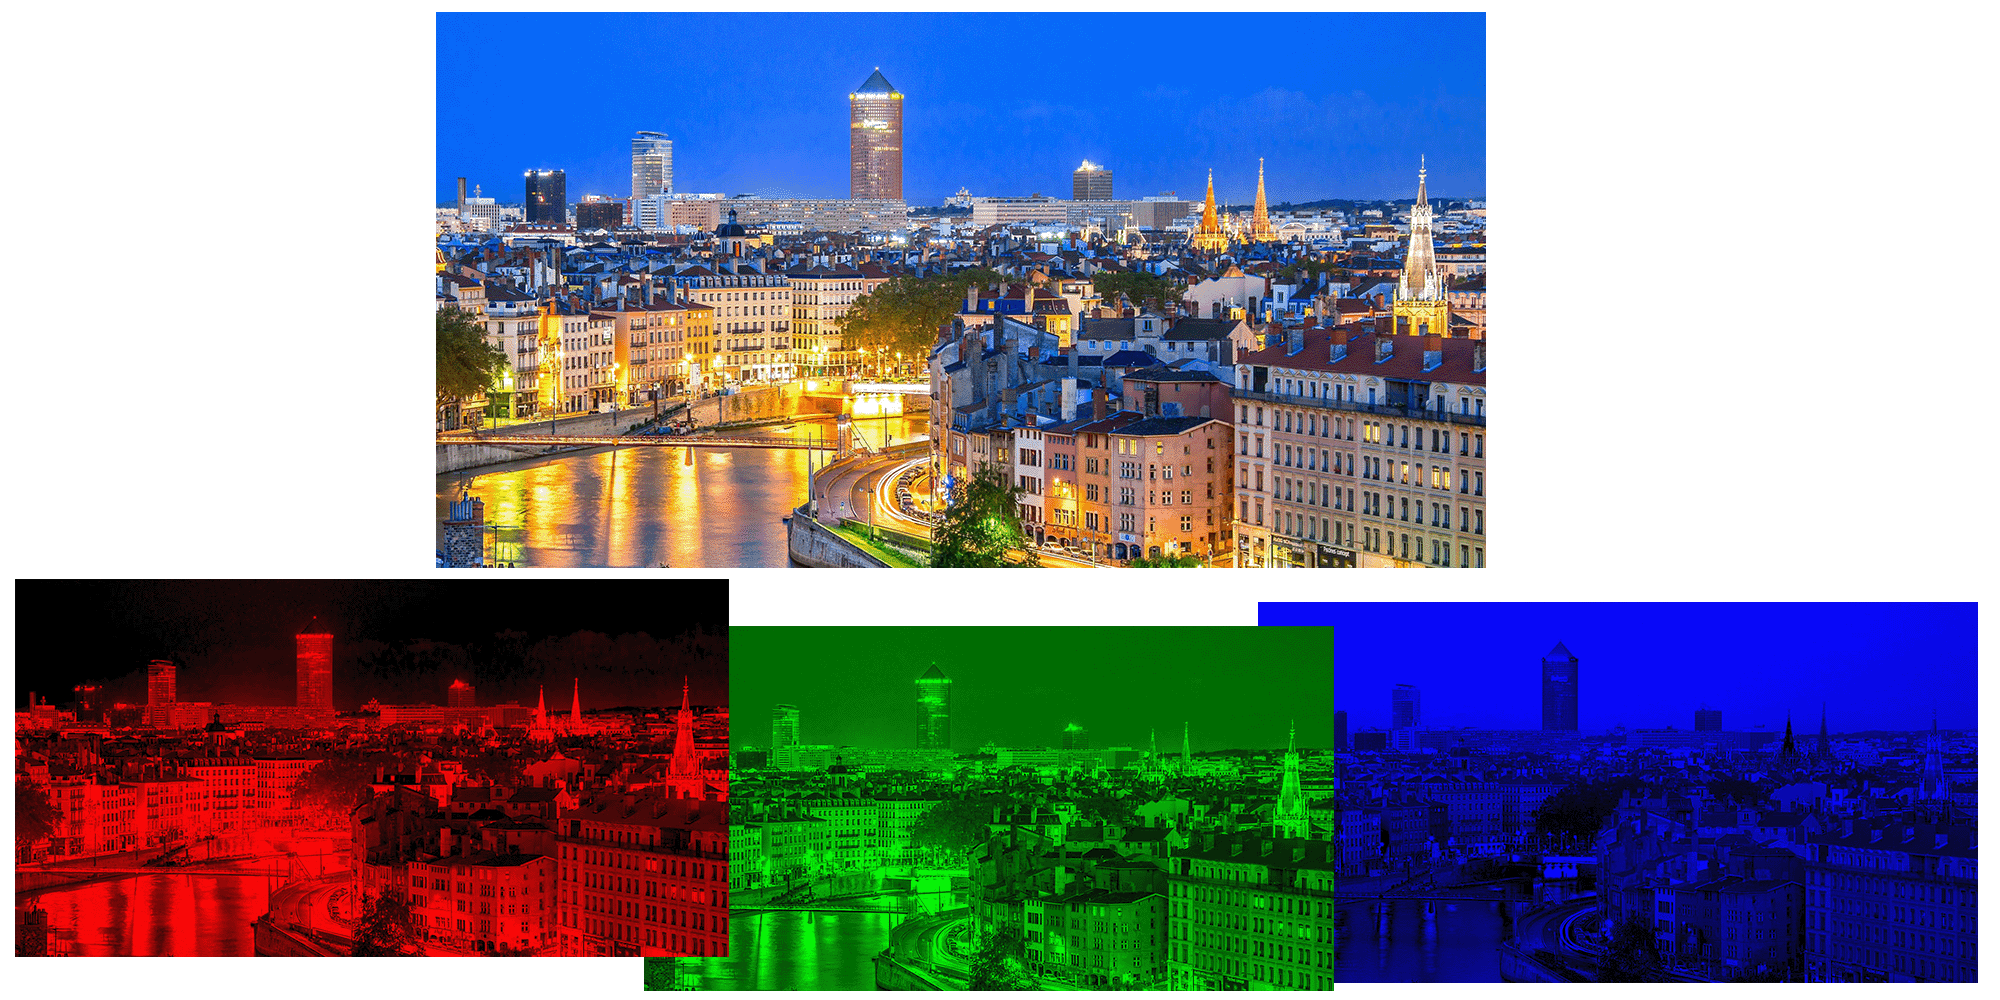
\includegraphics[width=0.8\textwidth]{img/diff_rgb.png}

\end{frame}

\begin{frame}
    \frametitle{La Représentation YCbCr}

    \begin{block}{Transformation YCbCr}
        \begin{align*}
            \varphi \colon \llbracket 0, 255 \rrbracket^3 & \rightarrow \llbracket 0, 255 \rrbracket \times \llbracket -128, 127 \rrbracket^2 \\
            X = (r, g, b) & \longmapsto
            TX = (Y, Cb, Cr)
          \end{align*}

      \vspace*{1em}

      $ T = 255\begin{pmatrix}
        K_r & K_r & K_b \\
        - \frac{1}{2} \cdot \frac{K_r}{1 - K_b} & - \frac{1}{2} \cdot \frac{K_g}{1 - K_b} & \frac{1}{2} \\
        \frac{1}{2} & - \frac{1}{2} \cdot \frac{K_g}{1 - K_r} & - \frac{1}{2} \cdot \frac{K_b}{1 - K_r} \\
      \end{pmatrix}$ et $K_r + K_g + K_b = 1$
    \end{block}
    \textit{Rq.} : En général $K_r = 0.299,\; K_g = 0.587, \; K_b = 0.114$

\end{frame}

\begin{frame}
    \frametitle{La Représentation YCbCr (2)}
    
    \centering
    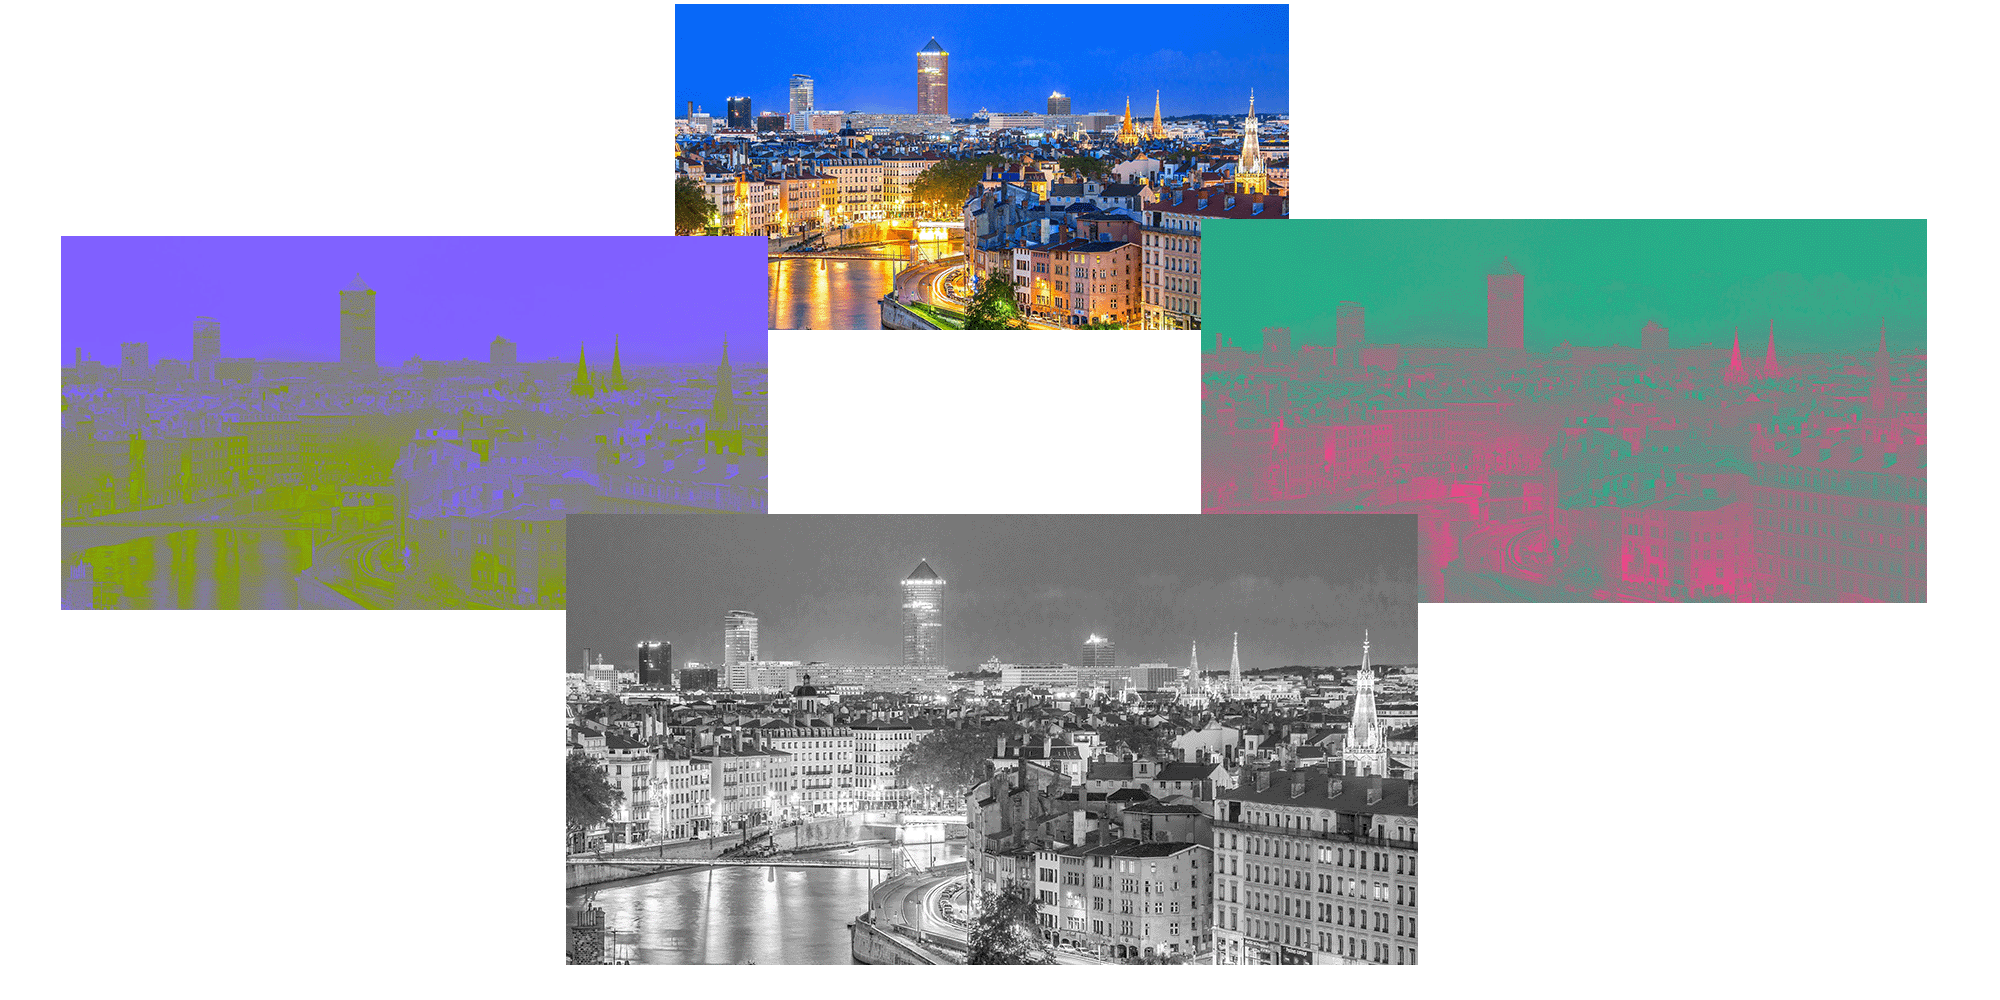
\includegraphics[width=\textwidth]{img/diff_YCbCr.png}

    \textbf{\OE{il} humain} $\rightarrow$ Y \textbf{prédomine}, Cb et Cr moins importants

\end{frame}

\begin{frame}
    \frametitle{Sous-\'Echantillonage}

    \begin{itemize}
        \item \textbf{Principe} : Cb, Cr moins importants -> \textbf{moyenner} ces valeurs sur \textbf{plusieurs pixels}
        \item Exemples de \textbf{sous-échantillonnages}: 
    \end{itemize}

    \centering
    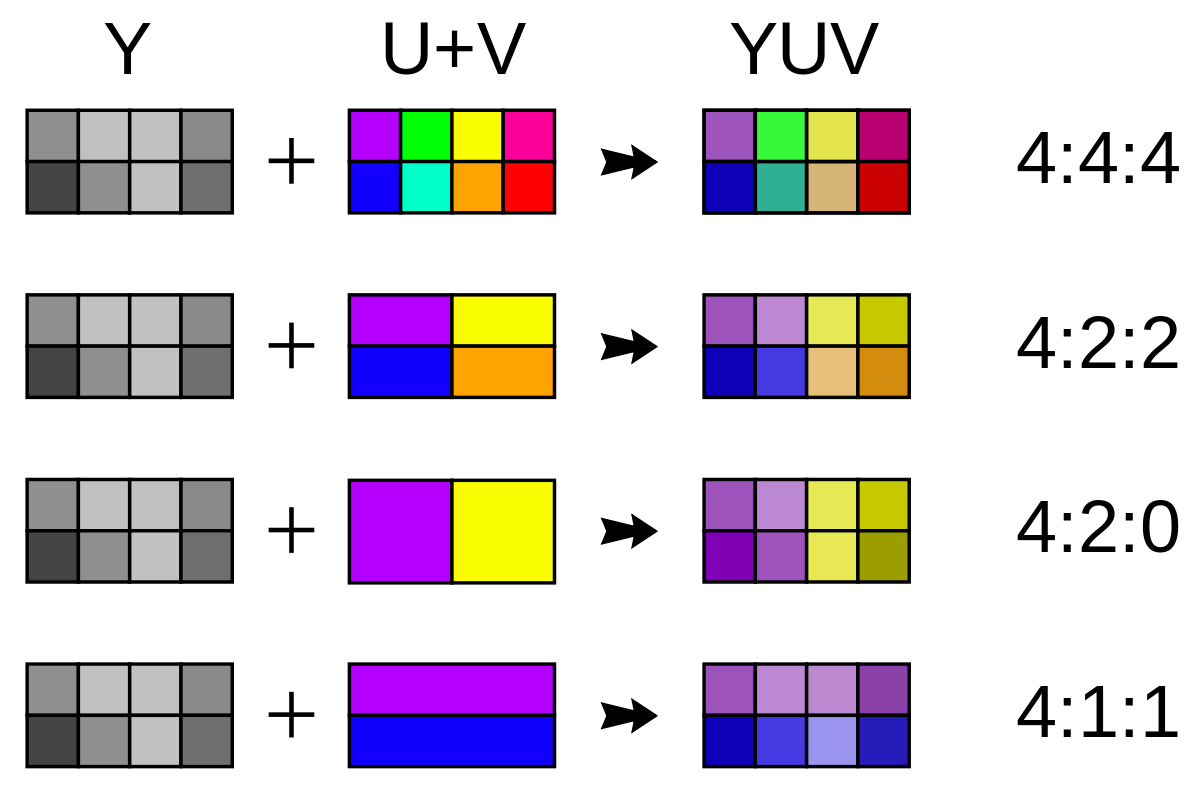
\includegraphics[width=0.8\textwidth]{img/chromaSubSampling.png}

\end{frame}

\begin{frame}
    \frametitle{DCT (transformée en cosinus discrète) (1)}
    \centering
    \begin{block}{Transformation DCT}
        \begin{align*}
            \psi \colon \mathbb{R}^N & \rightarrow \mathbb{R}^N\\
            (x_0, \dots, x_{N-1}) & \longmapsto
            \left( \sum_{n=0}^{N - 1} x_n \cos \left[ \frac{\pi}{N}(n + \frac{1}{2})k \right] \right)_{k \in \llbracket 0, N - 1 \rrbracket}
        \end{align*}
        On peut rendre la matrice associée à $\psi$ \textbf{orthogonale} en multipliant le terme $X_0$ par $\frac{1}{\sqrt{N}}$ et toute la matrice par $\sqrt{2/N}$.
    \end{block}
    2D-DCT $\rightarrow$ $\psi$ sur chaque lignes puis chaque colonne
\end{frame}

\begin{frame}
    \frametitle{DCT (2)}

    \begin{itemize}
        \item \textbf{"Continuité"} des images $\rightarrow$ peu de variations des \textbf{hautes fréquences}
        \item \textbf{Compactage} de l'énergie vers les \textbf{basses fréquences}
    \end{itemize}

    \centering
    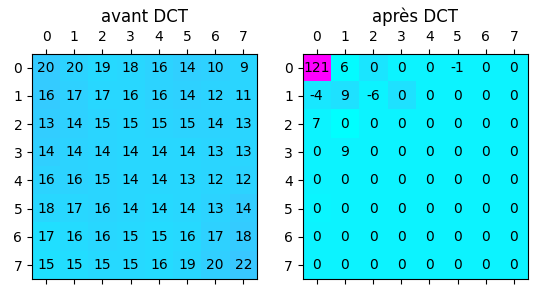
\includegraphics[width=\textwidth]{img/energyCompaction.png}

\end{frame}

\begin{frame}
    \frametitle{Quantification}

    \begin{itemize}
        \item Seule étape \textbf{avec perte} de la compression \textbf{JPEG}
        \item \textbf{Réduction} des coefficients
        \item \textbf{Différence} entre Y, Cb et Cr
        \item Fonction de quantification : \begin{align*}
            \varepsilon \colon \mathcal{M}_{8,8}(\mathbb{Z})^2 & \rightarrow \mathcal{M}_{8,8}(\mathbb{Z})\\
            Q, B & \longmapsto \lfloor B / Q \rfloor
        \end{align*}
        \item Souvent $Q$ dépend d'un \textbf{facteur de qualité} $q$
    \end{itemize}

\end{frame}

\begin{frame}
    \frametitle{Codage par plages (Run-Length Encoding)}

    \centering

    \begin{itemize}
        \item Tire son avantage des \textbf{répétitions} de symboles  
        \item Exemple : $$\underbrace{AAAA}_{4 \times A} \underbrace{B}_{1 \times B} \underbrace{CCC}_{3 \times C} \underbrace{BBBBBBB}_{7 \times B} \xrightarrow[RLE]{} A4B1C3B7$$
        $15$ caractères $\rightarrow$ $8$ caractères 
        \item Pour faire apparaître ces répétitions dans les \textbf{images}, lecture de la matrice en \textbf{zigzag}:
        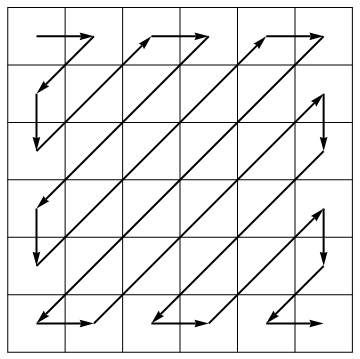
\includegraphics[width=0.2\textwidth]{img/zigzag.png}
    \end{itemize}

\end{frame}

\begin{frame}
    \frametitle{Exemple de Compression}

    \centering
    Image Original \\
    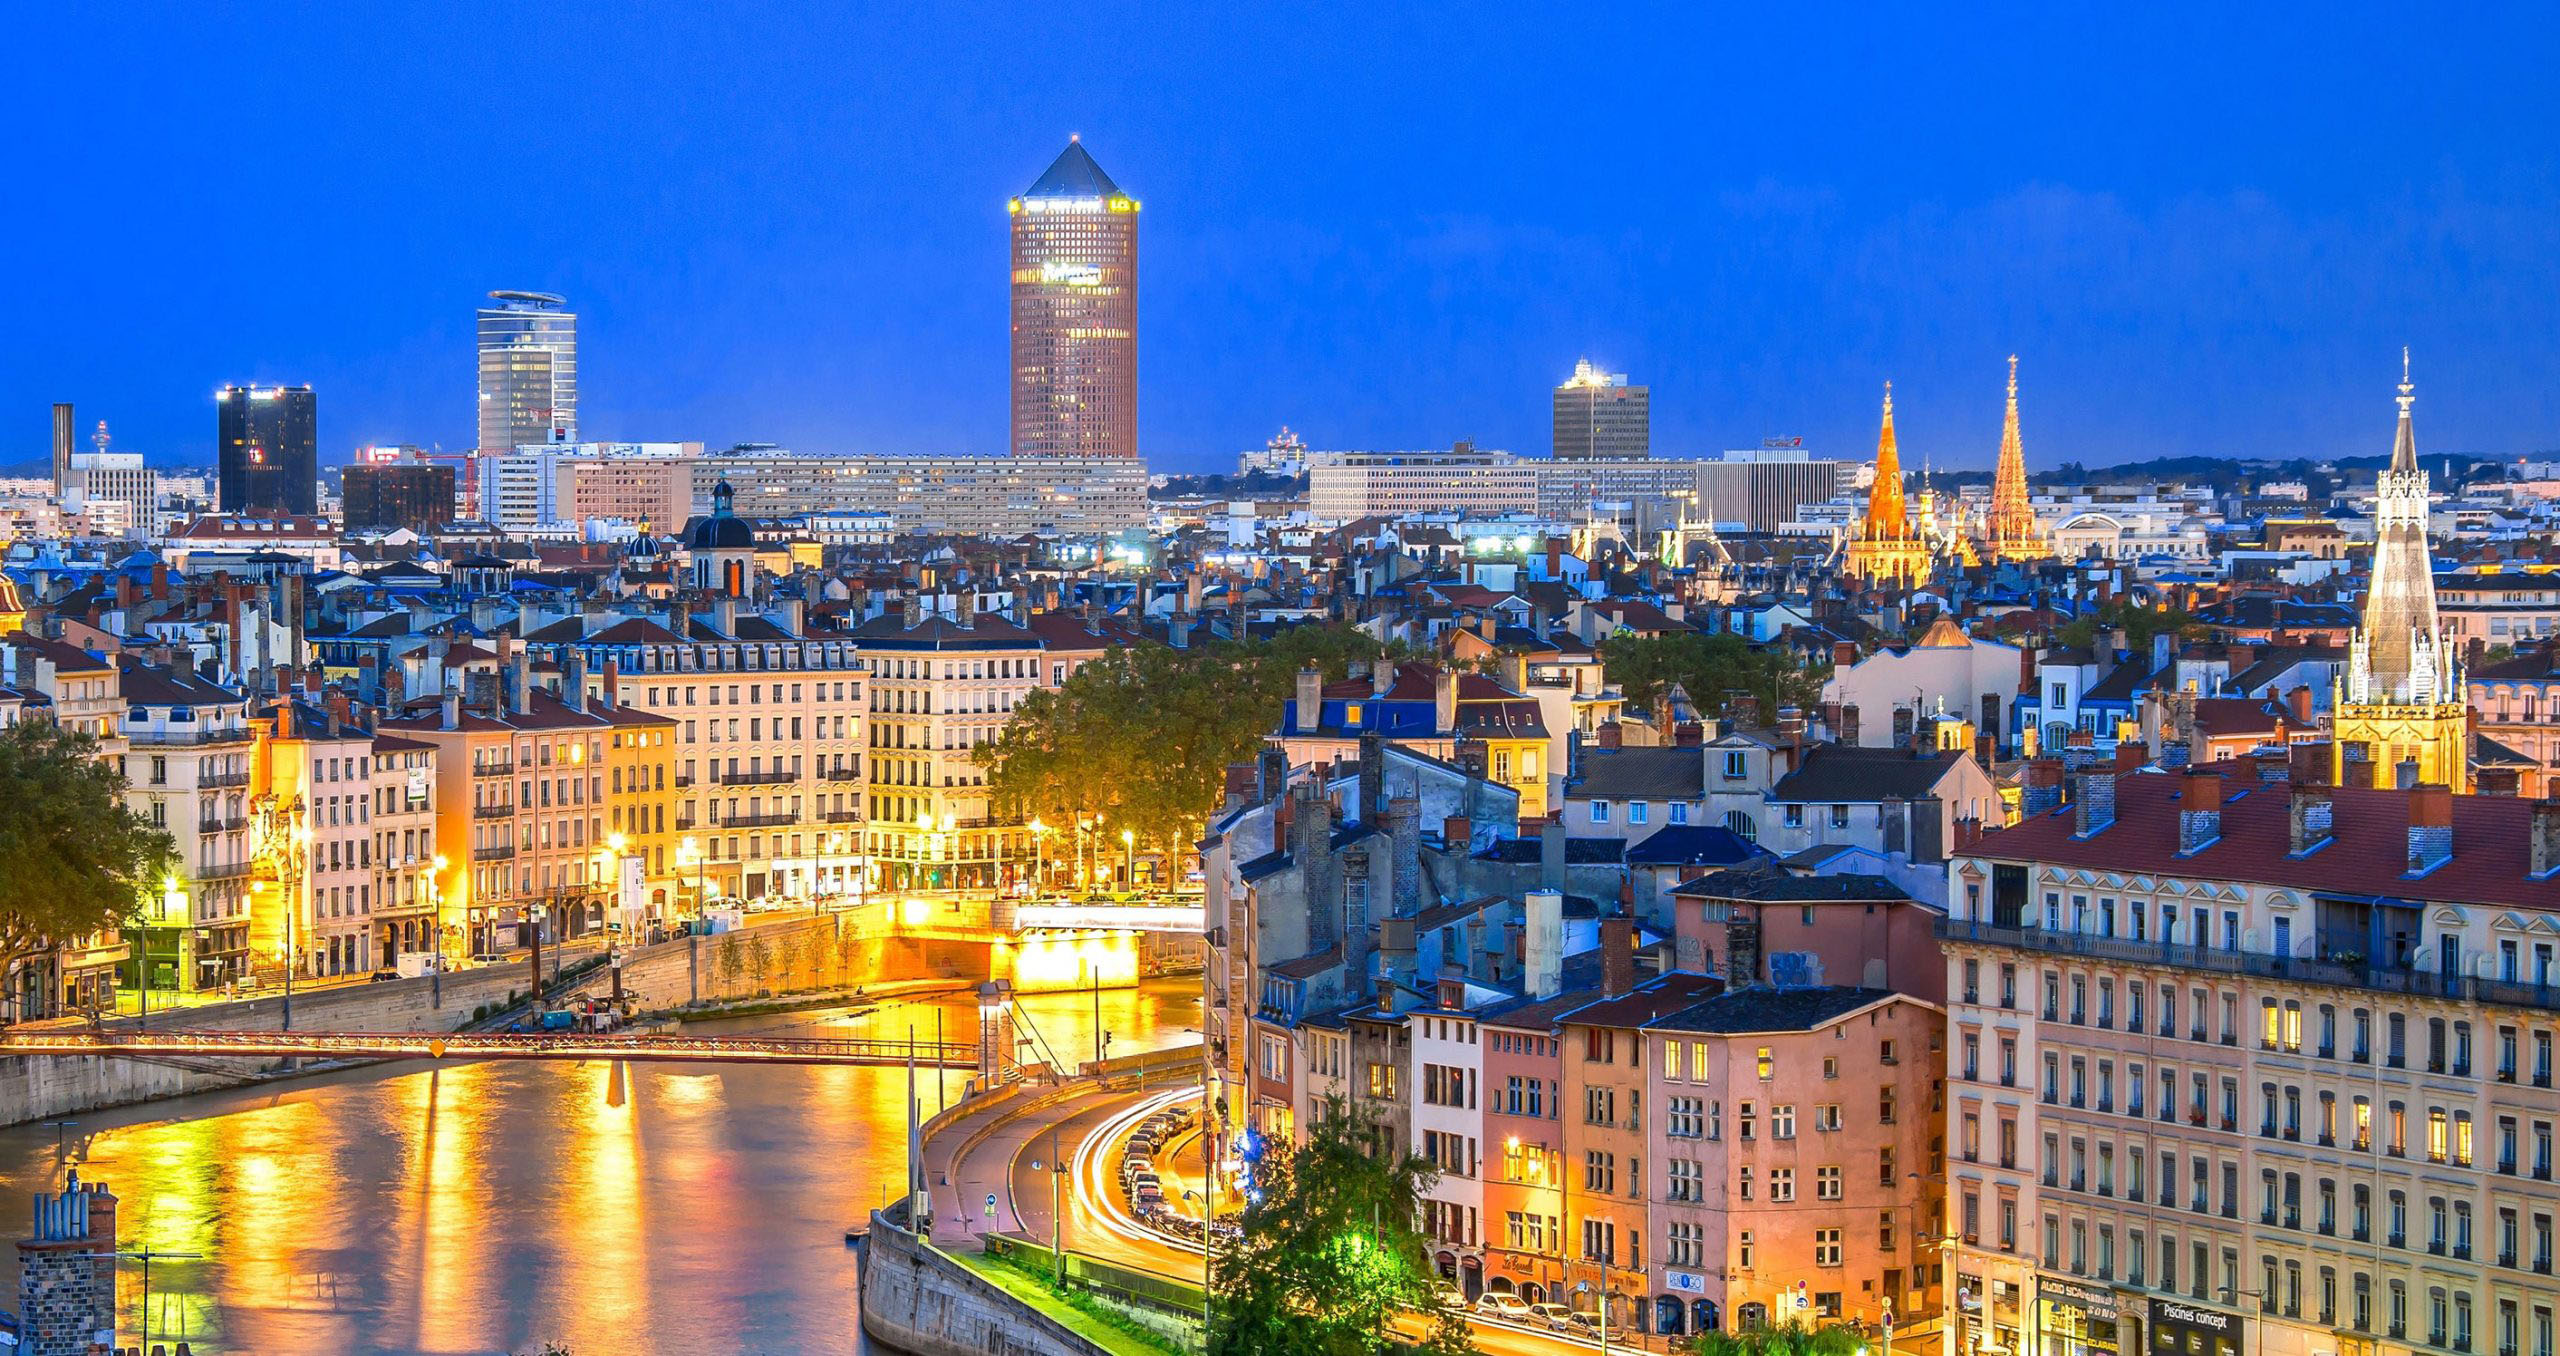
\includegraphics[width = 0.8\textwidth]{img/villeLyon.jpg} \\
    Taille : 10,3 Mo
\end{frame}

\begin{frame}
    \frametitle{Exemple de Compression}

    \centering
    Image Compressée ($q = 100$, $4:4:4$) (presque \textbf{lossless}) \\
    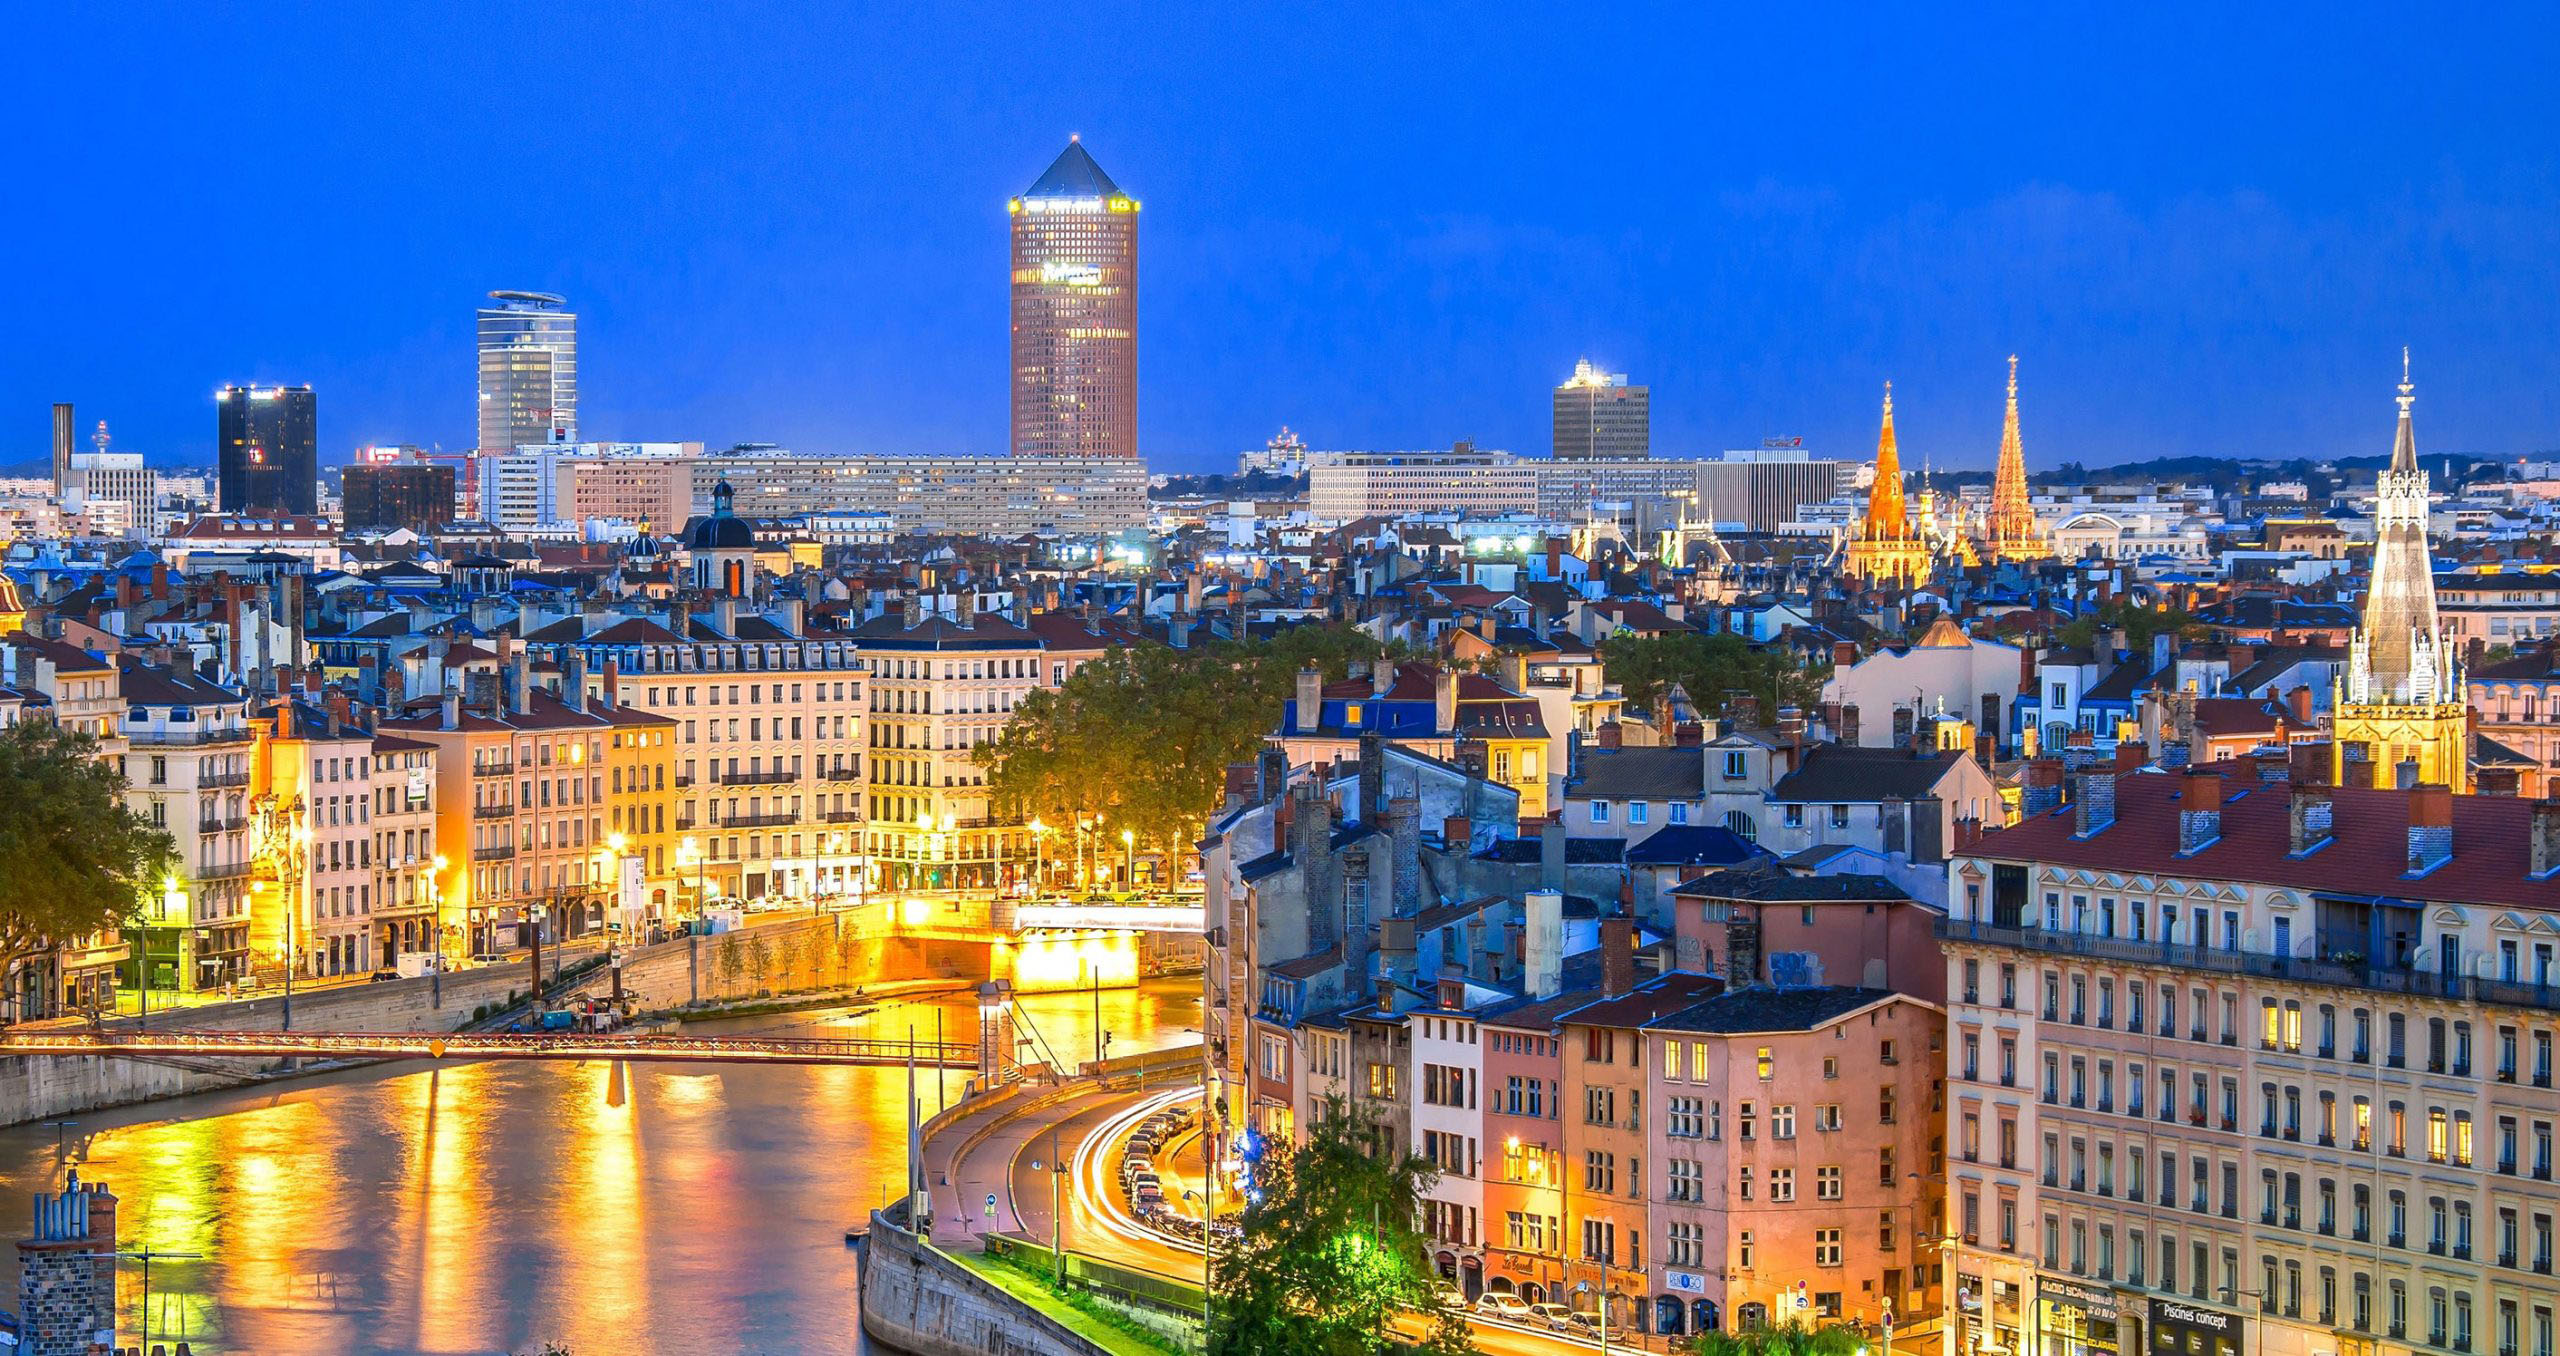
\includegraphics[width = 0.8\textwidth]{img/villeLyon.jpg} \\
    Taille : 2,2 Mo \\
    \textbf{Ratio} : $\eta = \frac{T_{init}}{T_{compres}} = 4.68 $

\end{frame}

\begin{frame}
    \frametitle{Exemple de Compression}

    \centering
    Image Compressée ($q = 50$, $4:2:2$) \\
    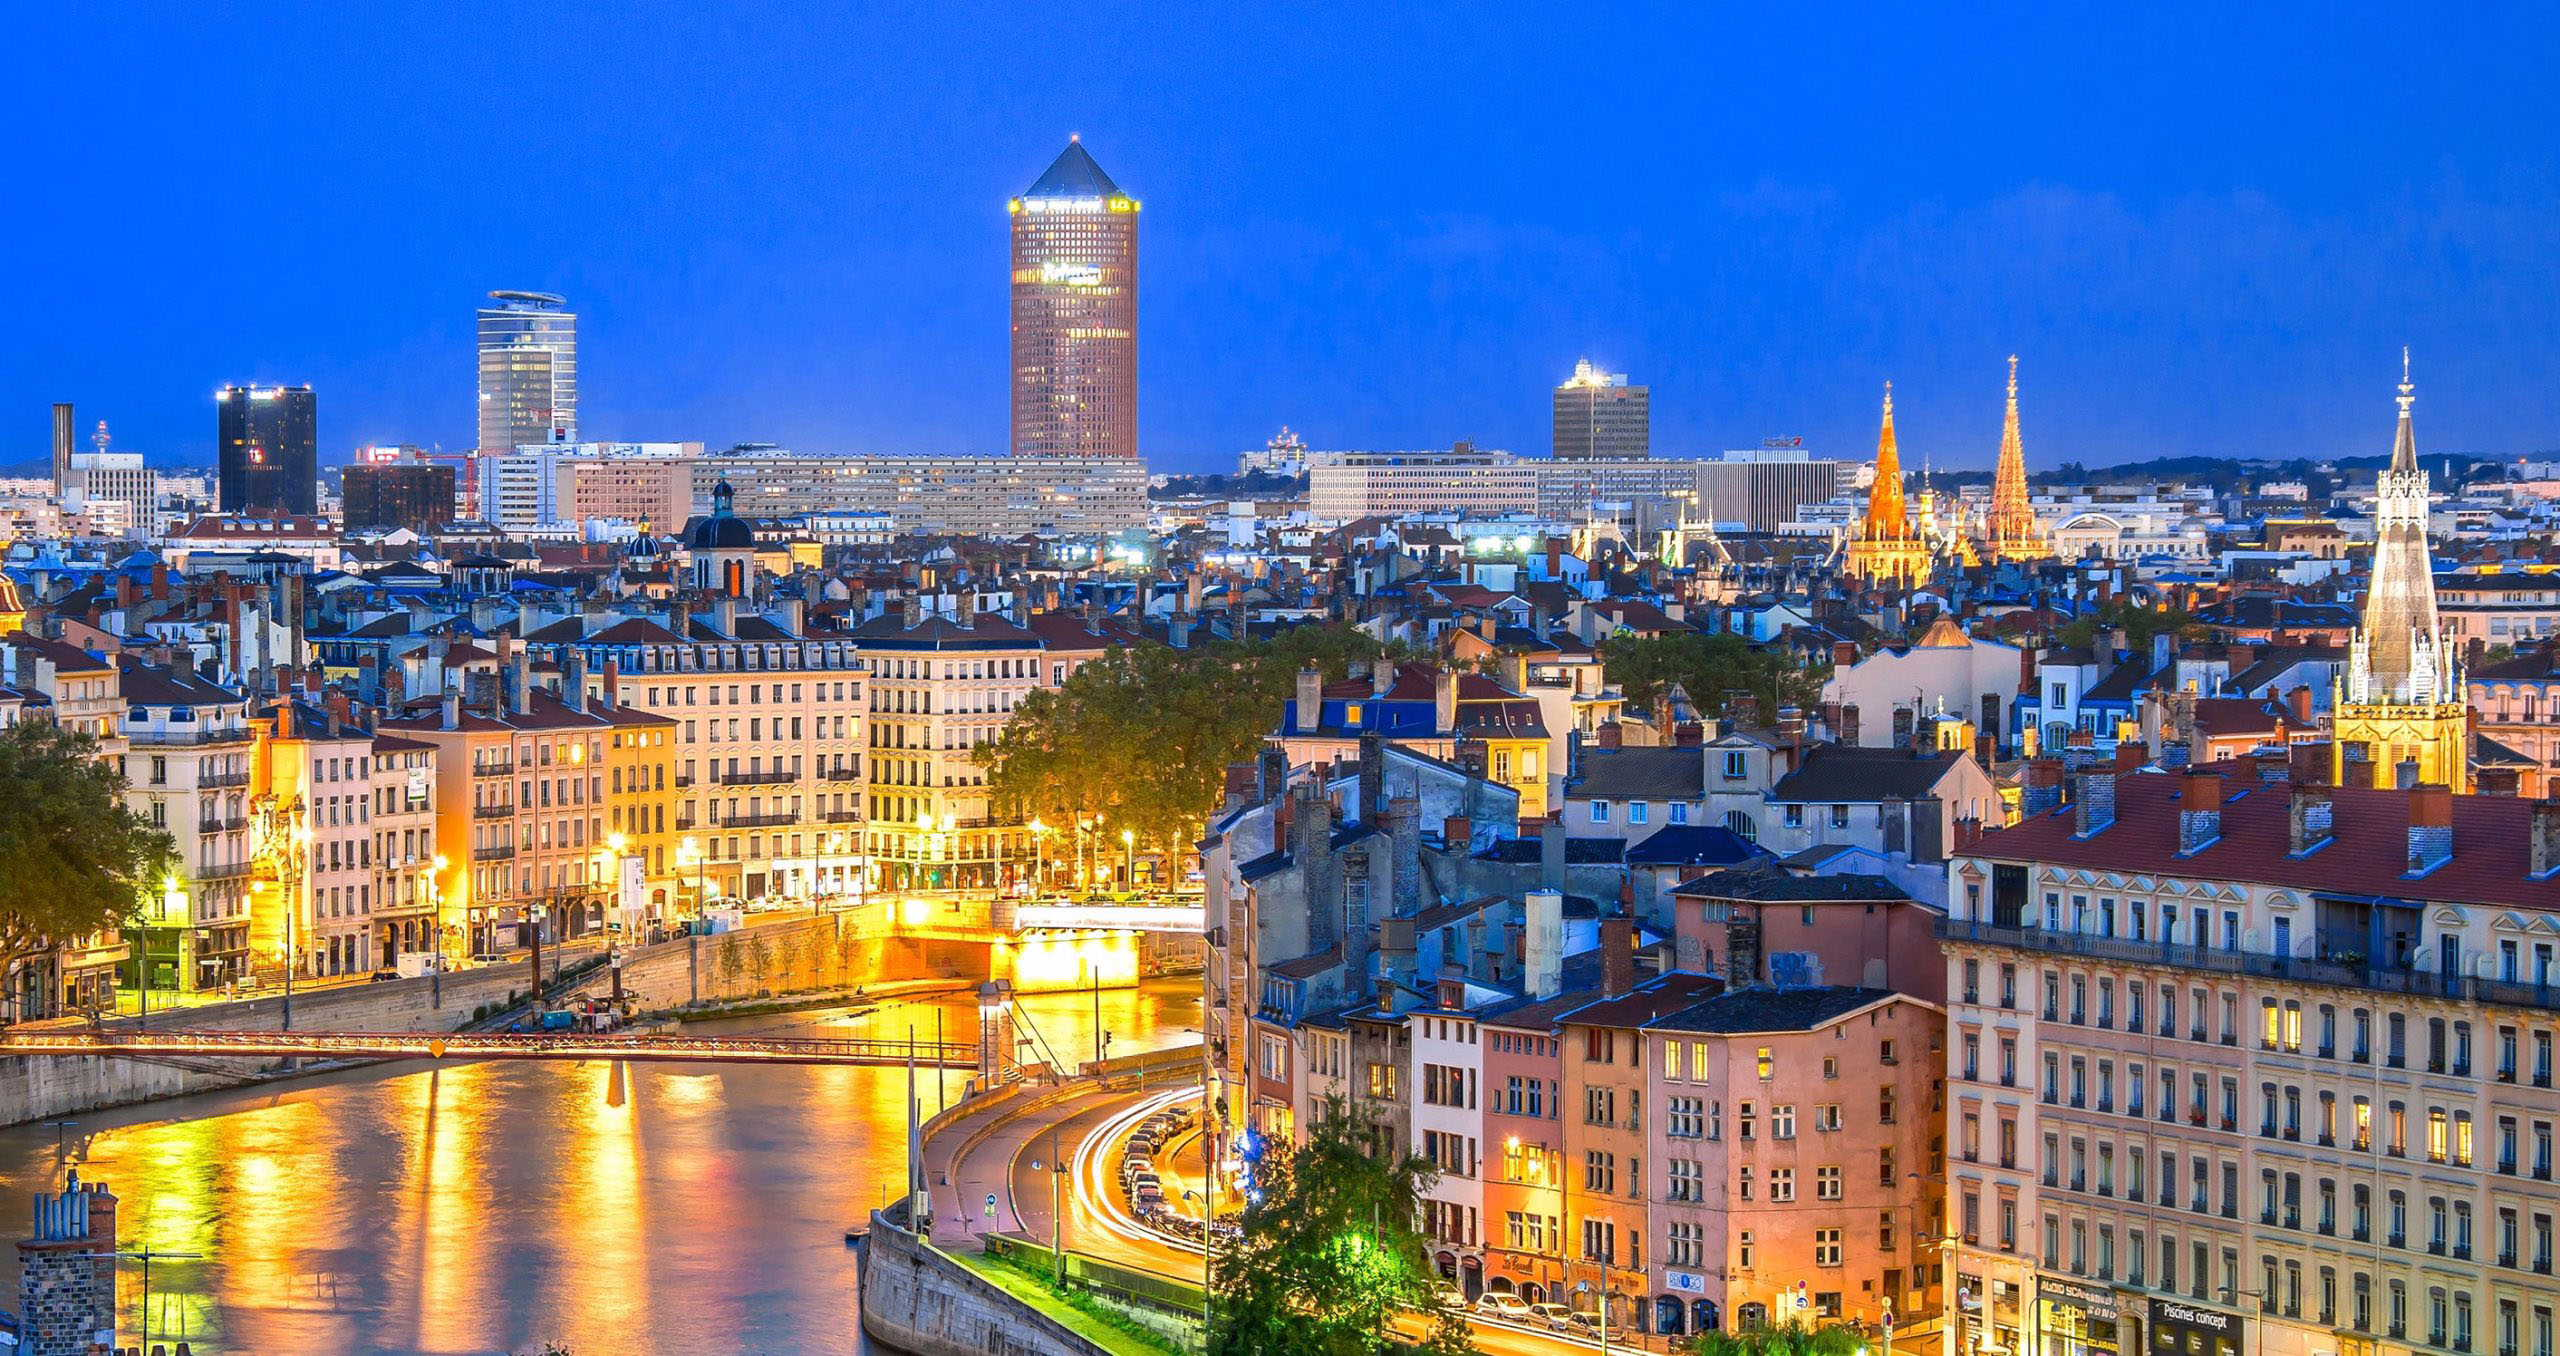
\includegraphics[width = 0.8\textwidth]{img/villeLyonMid.jpg} \\
    Taille : 519 Ko \\
    \textbf{Ratio} : $\eta = \frac{T_{init}}{T_{compres}} = 19.8$
    
\end{frame}

\begin{frame}
    \frametitle{Exemple de Compression}

    \centering
    Image Compressée ($q = 5$, $4:1:1$) \\
    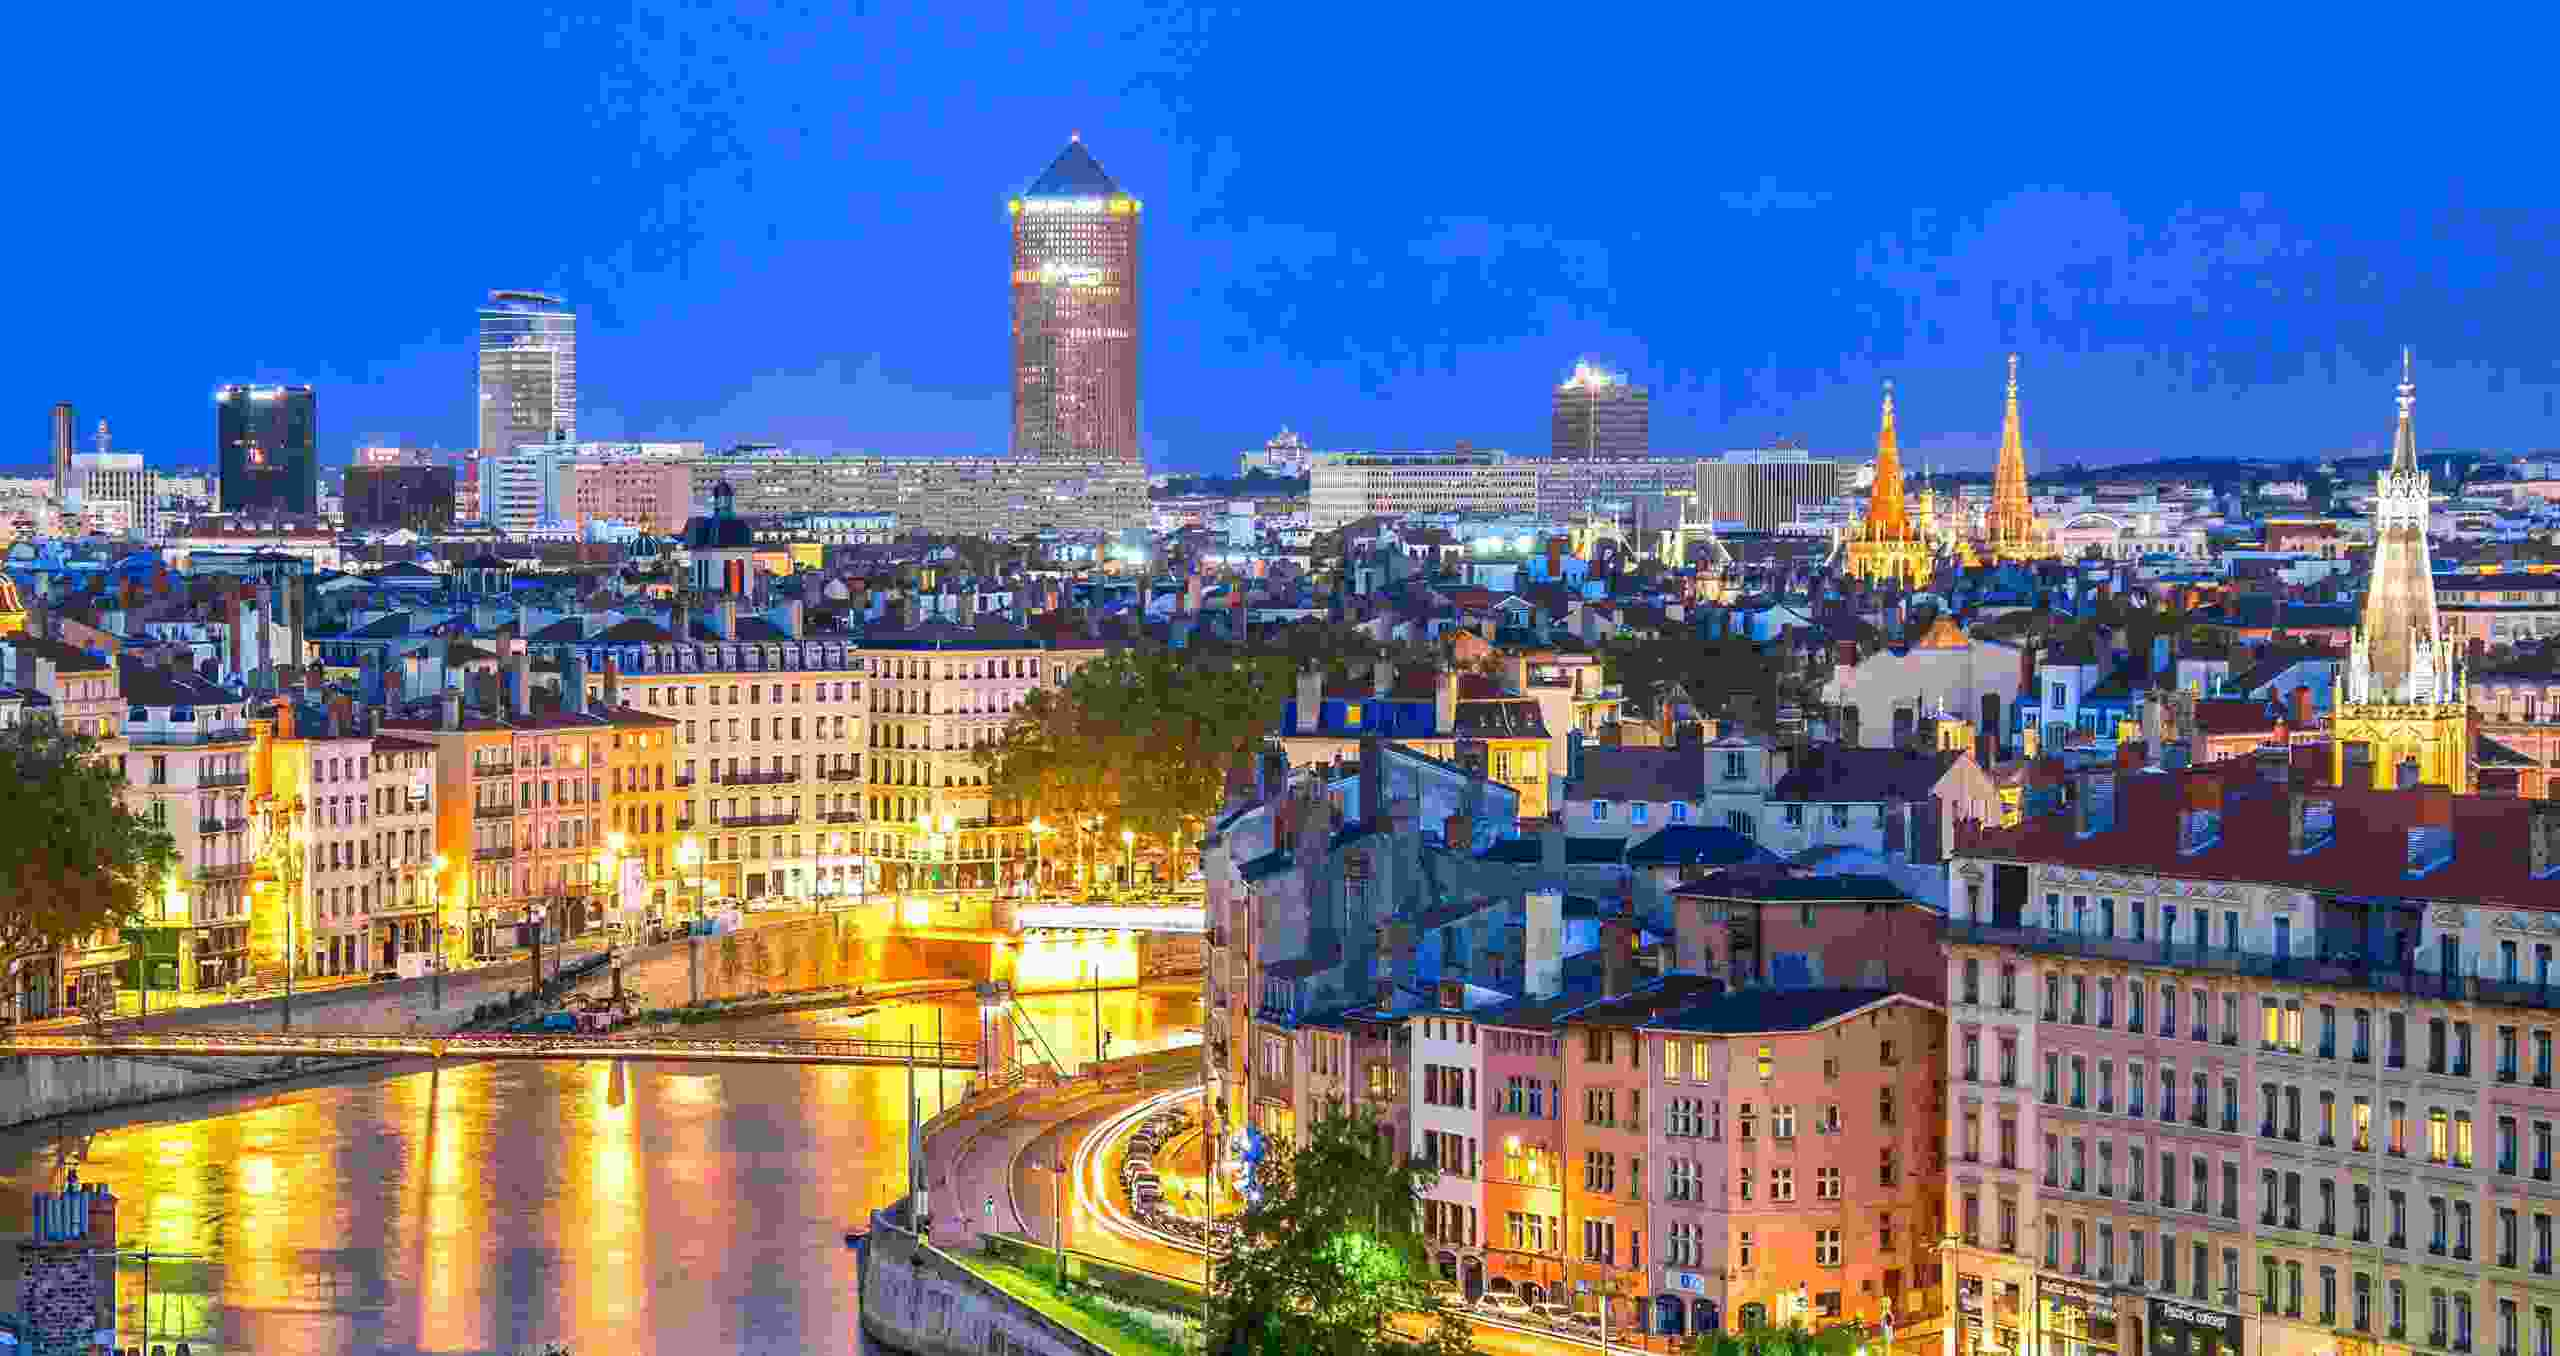
\includegraphics[width = 0.8\textwidth]{img/villeLyonLow.jpg} \\
    Taille : 77 Ko \\
    \textbf{Ratio} : $\eta = \frac{T_{init}}{T_{compres}} = 134$

\end{frame}

\begin{frame}
    \frametitle{Comparaison (1)}

    

\end{frame}

\begin{frame}
    \frametitle{Comparaison (2)}

    

\end{frame}
{
\setbeamercolor{background canvas}{bg=}
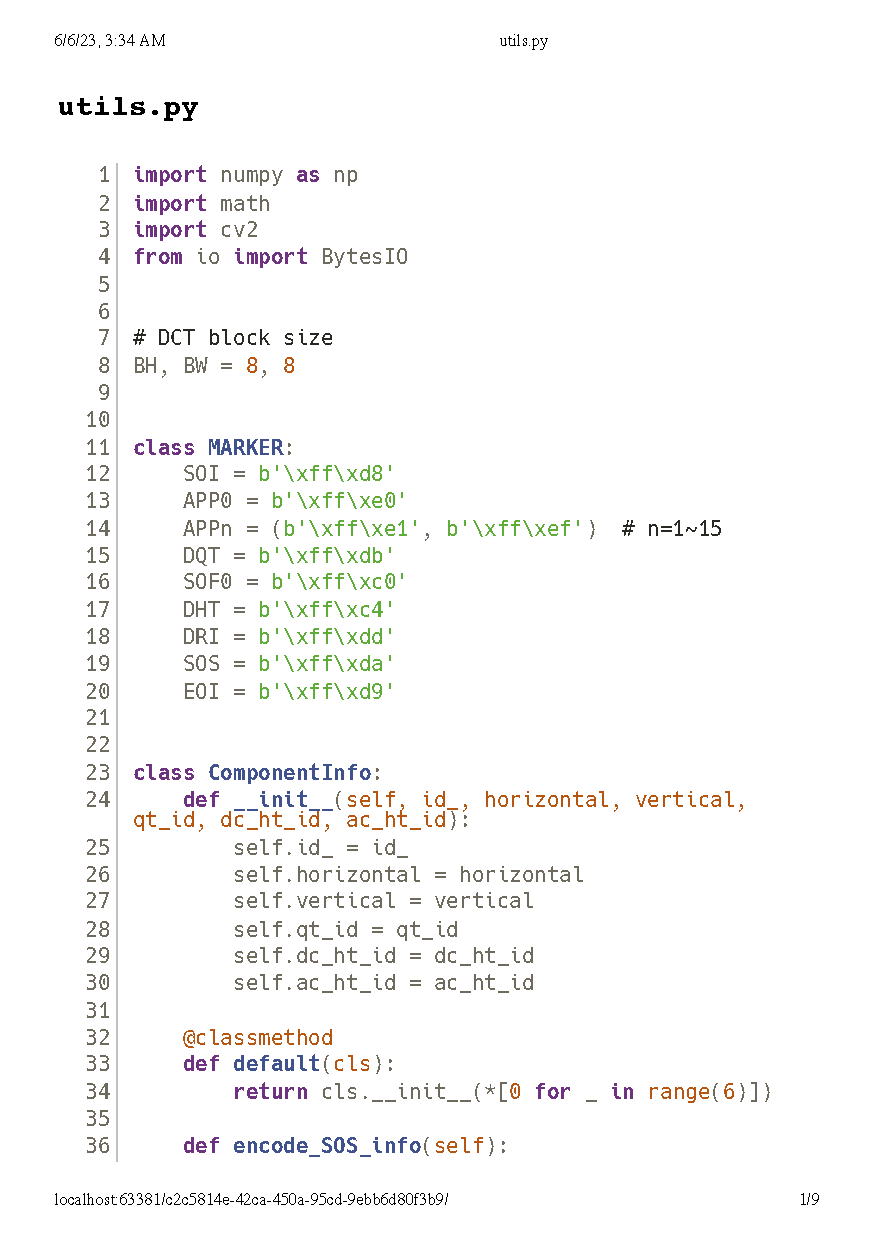
\includepdf[pages=1]{img/code/utils.py_compressed.pdf}
\includepdf[pages=2]{img/code/utils.py_compressed.pdf}
\includepdf[pages=3]{img/code/utils.py_compressed.pdf}
\includepdf[pages=4]{img/code/utils.py_compressed.pdf}
\includepdf[pages=5]{img/code/utils.py_compressed.pdf}
\includepdf[pages=6]{img/code/utils.py_compressed.pdf}
\includepdf[pages=7]{img/code/utils.py_compressed.pdf}
\includepdf[pages=8]{img/code/utils.py_compressed.pdf}
\includepdf[pages=9]{img/code/utils.py_compressed.pdf}
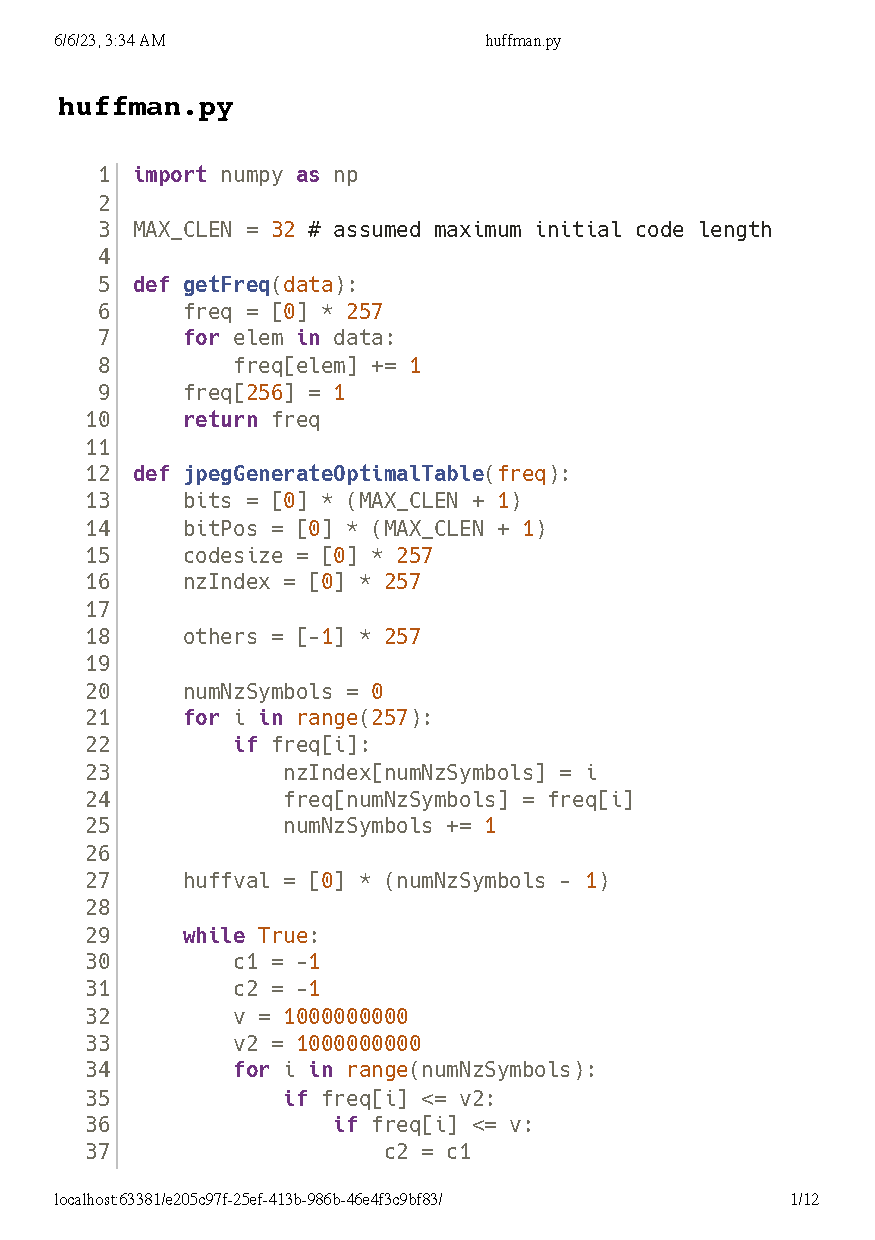
\includepdf[pages=1]{img/code/huffman.py_compressed.pdf}
\includepdf[pages=2]{img/code/huffman.py_compressed.pdf}
\includepdf[pages=3]{img/code/huffman.py_compressed.pdf}
\includepdf[pages=4]{img/code/huffman.py_compressed.pdf}
\includepdf[pages=5]{img/code/huffman.py_compressed.pdf}
\includepdf[pages=6]{img/code/huffman.py_compressed.pdf}
\includepdf[pages=7]{img/code/huffman.py_compressed.pdf}
\includepdf[pages=8]{img/code/huffman.py_compressed.pdf}
\includepdf[pages=9]{img/code/huffman.py_compressed.pdf}
\includepdf[pages=10]{img/code/huffman.py_compressed.pdf}
\includepdf[pages=11]{img/code/huffman.py_compressed.pdf}
\includepdf[pages=12]{img/code/huffman.py_compressed.pdf}
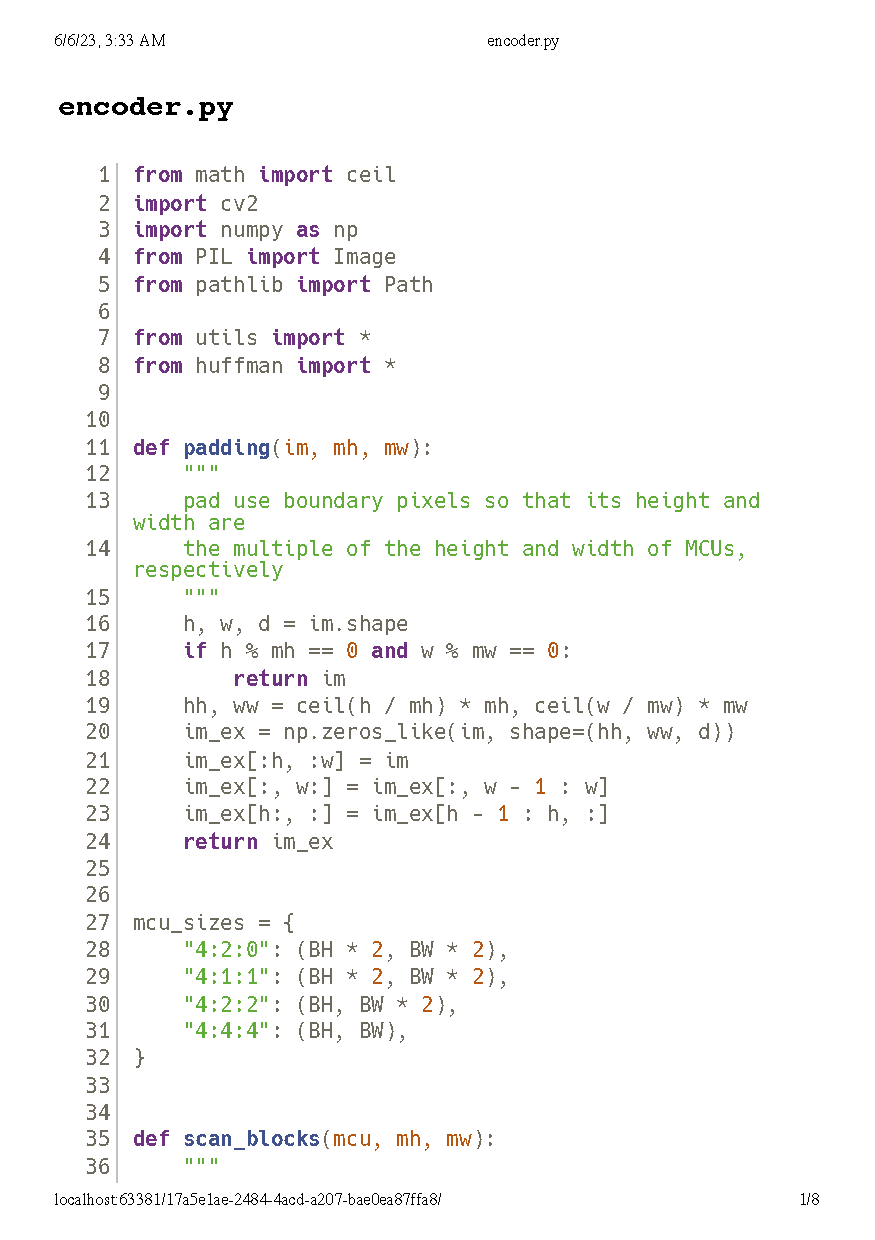
\includepdf[pages=1]{img/code/encoder.py_compressed.pdf}
\includepdf[pages=2]{img/code/encoder.py_compressed.pdf}
\includepdf[pages=3]{img/code/encoder.py_compressed.pdf}
\includepdf[pages=4]{img/code/encoder.py_compressed.pdf}
\includepdf[pages=5]{img/code/encoder.py_compressed.pdf}
\includepdf[pages=6]{img/code/encoder.py_compressed.pdf}
\includepdf[pages=7]{img/code/encoder.py_compressed.pdf}
\includepdf[pages=8]{img/code/encoder.py_compressed.pdf}
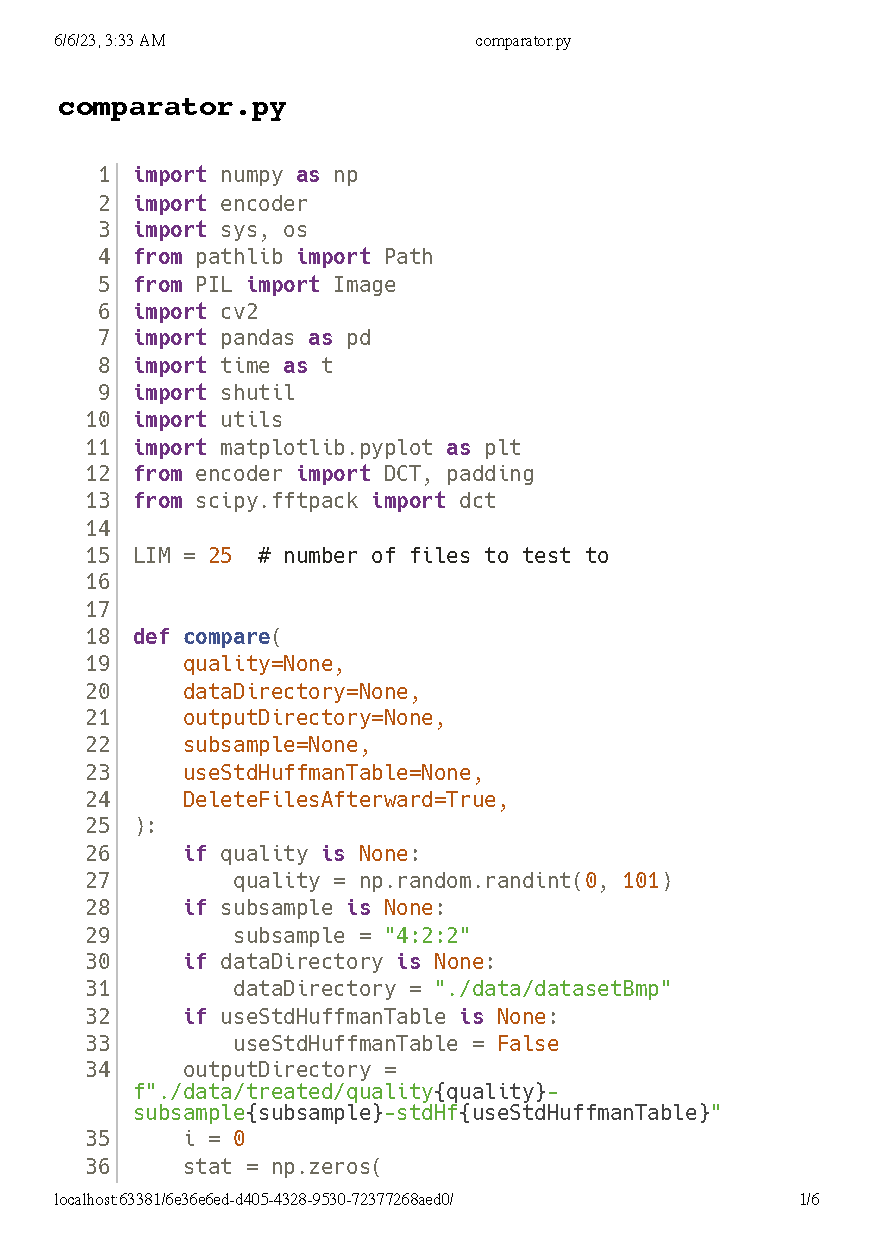
\includepdf[pages=1]{img/code/comparator.py_compressed.pdf}
\includepdf[pages=2]{img/code/comparator.py_compressed.pdf}
\includepdf[pages=3]{img/code/comparator.py_compressed.pdf}
\includepdf[pages=4]{img/code/comparator.py_compressed.pdf}
\includepdf[pages=5]{img/code/comparator.py_compressed.pdf}
\includepdf[pages=6]{img/code/comparator.py_compressed.pdf}
}

\end{document}